\documentclass[12pt,final,twoside]{article}
%%%%%%%%%%%%%%%%%%%%%%%%%%%%%%%%%%%%%%%%%%%%%%%%%%%%%%%%%%%%%
% Some credits:
% The template initially was created by Prof. Dr. Holger Karl/Uni Paderborn '2006
% and was expanded and updated by Dipl.-Inform. Stefan Heinrich/Uni Paderborn/Uni Hamburg since 2008.
% Suggestions for changes are always welcome.
%%%%%%%%%%%%%%%%%%%%%%%%%%%%%%%%%%%%%%%%%%%%%%%%%%%%%%%%%%%%%

\newcommand{\todowarn}{\color{yellow} TODO \color{red} TODO \color{blue} TODO}

% Meta information:
\newcommand{\trtitle}{Achieving results with untrained neural networks using Supermasks}
\newcommand{\trtype}{Independent Study Proposal}
\newcommand{\trcourseofstudies}{Intelligent Adaptive Systems} %{Bioinformatik} 
\newcommand{\trauthor}{Vincent Rolfs}
\newcommand{\trauthortitle}{} %{Dipl.-Inform.\ }
\newcommand{\tremail}{vincent.rolfs@studium.uni-hamburg.de}
\newcommand{\trmatrikelnummer}{6789106}
%\newcommand{\trstrasse}{Streetname 42}
%\newcommand{\trort}{22527 Hamburg}
\newcommand{\trgutachterA}{\href{mailto:wermter@informatik.uni-hamburg.de}{Prof. Dr. S. Wermter}}
\newcommand{\trgutachterB}{\href{mailto:matthias.kerzel@informatik.uni-hamburg.de}{Dr. M. Kerzel}}
%\newcommand{\trbetreuung}{\href{mailto:tbd@informatik.uni-hamburg.de}{Dipl.-Inform. To Be Defined}}
\newcommand{\trfach}{Knowledge Technology, WTM}
\newcommand{\trdate}{\todowarn}
\newcommand{\trkeywords}{}

%%%%%%%%%%%%%%%%%%%%%%%%%%%%%%%%%%%%%%%%%%%%%%%%%%%%%%%%%%%%%
% Languages:

% If the thesis is written in English:
\usepackage[english]{babel}                         
\selectlanguage{english}

%%%%%%%%%%%%%%%%%%%%%%%%%%%%%%%%%%%%%%%%%%%%%%%%%%%%%%%%%%%%%
% Bind packages:

\usepackage[backend=biber,bibencoding=utf8]{biblatex}
\addbibresource{bibliography.bib} 

\usepackage{amsfonts}                   % AMS Math Packet (Fonts)
\usepackage{amsmath}                    % AMS Math Packet
\usepackage{amssymb}                    % Additional mathematical symbols
\usepackage{amsthm}
\usepackage{color}                      % Enables defining of colours via \definecolor
\definecolor{uhhRed}{RGB}{226,0,26}     % Official Uni Hamburg Red
\definecolor{uhhGrey}{RGB}{136,136,136} % Official Uni Hamburg Grey
\definecolor{uhhLightGrey}{RGB}{220, 220, 220}
\usepackage{fancyhdr}                   % Packet for nicer headers
\usepackage[body={5.8in,9in}]{geometry} % Type area (size, margins...)
\usepackage{booktabs, makecell} % tables
\renewcommand\theadfont{\bfseries}

\usepackage{float}

%\geometry{a4paper,outer=3.35cm}        % !!!Release version (Normal margins)
%\geometry{a4paper,outer=2.5cm}         % !!!Print version (Additional margin on the left for the binding)
%\geometry{a4paper}                     % !!!Proofread version (Additional margin on the right for corrections)
\geometry{a4paper,outer=3.15cm}         % !!!Draft version (Same margins on left and right)
%\geometry{paperheight=10.0in,paperwidth=6.4in,top=0.51in,left=0.3in}  % !!!Developer version (Minimal margins)

\usepackage{graphicx}                   % Inclusion of graphics

\usepackage{enumerate}
\usepackage{enumitem}[labelsep=8pt ,labelindent=3cm ,itemindent=3cm ,leftmargin=3cm ,listparindent=3cm]
%
%\newlist{phases}{enumerate}{1}
%\setlist[phases]{label=Phase \arabic*:}

%%%%%%%%%%%%%%%%%%%%%%%%%%%%%%%%%%%%%%%%%%%%%%%%%%%%%%%%%%%%%
% PDF Information und Definitions:
\author{\trauthor}

\ifx\pdftexversion\undefined
\usepackage{hyperref}
\else
\usepackage[colorlinks=false,           % link is colores (true) or has colored frame (false)
            linkcolor=uhhRed,           % case colorlinks=true: define color.
            urlcolor=uhhRed,
            citecolor=uhhRed,
            bookmarks,                  % Place bookmarks erstellen
            bookmarksopen=true,         % Bookmarks will be shown at start (true/false)
            pdfpagemode=UseOutlines,    
            bookmarksopenlevel=1,       % Define the depth of shown links
            bookmarksnumbered,          % Numbers of chapers in Bookmarks
            pdftitle={\trtitle},
            pdfsubject={\trtype},
            pdfkeywords={\trkeywords},
            pdfauthor={\trauthor},
            plainpages=false
            ]{hyperref}
\fi

\ifx\pdftexversion\undefined
\else
\pdfoutput=1                            % Disable PDF-Output
\pdfimageresolution=1200
\pdfcompresslevel=2                     % 0 = no compression, 9 = strongest compression
\fi

%%%%%%%%%%%%%%%%%%%%%%%%%%%%%%%%%%%%%%%%%%%%%%%%%%%%%%%%%%%%%
% Configurationen:

\hyphenation{whe-ther}                  % Manually use: "\-" in a word: Staats\-ver\-trag

\DeclareGraphicsExtensions{.pdf,.svg,.jpg,.png,.eps} % first try pdf, then eps, png and jpg
\graphicspath{{./src/}}                 % Path to a folder where all pictures are located
\pagestyle{fancy}                       % Use nicer header and footer

% Redefine the environments for floating objects:
\setcounter{topnumber}{3}
\setcounter{bottomnumber}{2}
\setcounter{totalnumber}{4}
\renewcommand{\topfraction}{0.9}        %Standard: 0.7
\renewcommand{\bottomfraction}{0.5}     %Standard: 0.3
\renewcommand{\textfraction}{0.1}       %Standard: 0.2
\renewcommand{\floatpagefraction}{0.8}  %Standard: 0.5

% Tables with a nicer padding:
\renewcommand{\arraystretch}{1.2}

% Chapter and Sections will not be written in capitals
%\renewcommand{\chaptermark}[1]{\markboth{\chaptername \ \thechapter.\ #1}{}}
\renewcommand{\sectionmark}[1]{\markright{\thesection.\ #1}}

%%%%%%%%%%%%%%%%%%%%%%%%%%%%
% Additional 'theorem' and 'definition' blocks:
\theoremstyle{plain}
\newtheorem{theorem}{Theorem}[section]
\newtheorem{axiom}{Axiom}[section]

\theoremstyle{definition}
\newtheorem{definition}{Definition}[section]

%Additional types of axioms:
\newtheorem{lemma}[axiom]{Lemma}
\newtheorem{observation}[axiom]{Observation}

%Additional types of definitions:
\theoremstyle{remark}
\newtheorem{remark}[definition]{Remark}

% Custom theorem name
% https://tex.stackexchange.com/questions/12913/customizing-theorem-name
\newtheoremstyle{named}{}{}{\itshape}{}{\bfseries}{.}{.5em}{\thmnote{#3}}
\theoremstyle{named}
\newtheorem*{namedtheorem}{Theorem}

%%%%%%%%%%%%%%%%%%%%%%%%%%%%
% Provides TODOs within the margin:
\newcommand{\TODO}[1]{\marginpar{\emph{\small{{\bf TODO: } #1}}}}

%%%%%%%%%%%%%%%%%%%%%%%%%%%%
% Abbreviations and mathematical symbols


%%%%%%%%%%%%%%%%%%%%%%%%%%%%%%%%%%%%%%%%%%%%%%%%%%%%%%%%%%%%%
% Document:

\begin{document}

\pagenumbering{Roman}                   % Roman pagenumbering for lists and meta pages
\renewcommand{\headheight}{14.5pt}      % Size of headings

\thispagestyle{empty}
\fancyhead[LO,RE]{}                     % Define the header style for the meta pages

%%%%%%%%%%%%%%%%%%%%%%%%%%%%
% Cover sheet

\begin{titlepage}
%---Possibility 1:
    \begin{flushleft}
        
\includegraphics[width=85mm]{uhhLogoL.pdf}\\
    \end{flushleft}
%---Possibility 2:
%\includegraphics*[width=0.09\textwidth]{uhhIconR_}
%\parbox[c]{10cm}{
%    \begin{center}
%    Universit\"at Hamburg --- MIN-Fakult\"at\\
%    \trfachgruppe
%    \end{center}
%    }\hfill
%\includegraphics*[width=0.09\textwidth]{infIcon_}
%\vspace{0.2cm}
%---
    \rule{\textwidth}{0.4pt}
        \newline
        \vspace{2.0cm}
        \begin{center}
          \LARGE \textbf{\trtitle}
        \end{center}
    \vspace{2.0cm}
    \begin{center}
      \textbf{\trtype}\\
      %am Fachgebiet \trfach\\
      im Arbeitsbereich \trfach\\
      \trgutachterA\medskip\\
      Department Informatik\\
      MIN-Fakult\"at\\
      Universit\"at Hamburg \\[0.5cm]
      vorgelegt von \\
      \textbf{\trauthortitle\href{mailto:\tremail}{\trauthor}}\\
      am\\
      \trdate
    \end{center}
    \vspace{1cm}
    \begin{center}
    \begin{tabular}{ll}
    Gutachter: & \trgutachterA \\
                   & \trgutachterB \\
    %Betreuung: & \trbetreuung \\    	% Adviser are not allowed to demand getting credited, but are happy getting credited by the students initiative
    \end{tabular}
    \end{center}
    \vfill
    \begin{tabular}{l}
    \trauthor \\
    Matrikelnummer:  \trmatrikelnummer \\
    %\trstrasse \\
    %\trort
    \end{tabular}
    \newline
    \rule{\textwidth}{0.4pt}
    \newpage 
\end{titlepage}

%backsite of cover sheet is empty!
%\thispagestyle{empty}
%\hspace{1cm}
%\newpage

%%%%%%%%%%%%%%%%%%%%%%%%%%%%
% Lists:
%\setcounter{tocdepth}{1}               % depth of the table of contents (for BSc and MSc Thesis 1 is recommented)
\fancyhead[LE,RO]{\it Contents}
\tableofcontents
\newpage

\fancyhead[LE]{\it \rightmark}           % Define the header style for the text pages
\fancyhead[RO]{\it \rightmark}          % Define the header style for the text pages
\fancyhead[LO,RE]{}                     % Define the header style for the text pages

%%%%%%%%%%%%%%%%%%%%%%%%%%%%
% The content will be included here:
\pagenumbering{arabic}

\section{Introduction}
Interest in decreasing the size of neural networks that are used to solve certain problems has existed since at least the year 1990 \cite{braindamage}. Different methods have been proposed that can be used to achieve a decrease in network size of up to 90\% while retaining performance \cite{braindamage} \cite{learning-weights-connections} \cite{brainsurgeon} \cite{pruning-filters}.

This has multiple advantages, which can be classified according to the type of pruning that is applied. If the network is pruned after training while otherwise keeping the trained weights constant, this may result in reduced storage size, less energy consumption and faster computation during the application phase \cite{lottery}. If it is possible to retrain the smaller network from scratch, this may result in less overfitting because the number of parameters has decreased  \cite{learning-weights-connections}. And if a smaller but still effective network topology can be chosen \textit{before training}, this can reduce the training time, because less parameters have to be optimized.

However, conventional pruning techniques have the problem that, when retraining from scratch on the smaller topology, the performance gets considerably worse \cite{lottery}. These pruning techniques are only amenable for pruning the weights computed by an inital training run, and do not work well if the aim is to retrain once again on the smaller topology. Therefore, they cannot be used to choose a good topology before the training starts, because the correct parameters for the smaller network can only be discovered by training the larger network.

In contrast to this negative state of affairs, in their paper "The Lottery Ticket Hypothesis: Finding Sparse, Trainable Neural Networks" \cite{lottery}, the authors present a hypothesis that essentially claims that pre-training pruning nonetheless has a lot of potential:

\begin{namedtheorem}[The Lottery Ticket Hypothesis \cite{lottery}]
A randomly-initialized, dense neural network contains a subnetwork that is initialized such that -- when trained in isolation -- it can match the test accuracy of the original network after training for at most the same number of iterations.
\end{namedtheorem}

The authors further show that the subnetwork mentioned in the hypothesis can be uncovered by training the dense network and then setting a percentage $p\%$ of the parameters with smallest magnitude to zero (and freezing them, so that they are not trained anymore). If the remaining parameters are then set to their inital values (the random values they had before the training started), and one retrains the smaller network starting with these initial values, then the training time will usually be less and the test performance better compared to the original, dense, trained network \cite{lottery}.

It is imperative here that the non-frozen parameters are reset to their \textit{initial}, random values, not newly chosen random values. If the latter is chosen, the performance is much worse and the "Lottery Ticket" has not been uncovered \cite{lottery}. In other words, we should not only search for efficient network topologies, but also for good initial values.

This curious fact has been further investigated by Zhou et al.\ \cite{supermask}. They realized that the subnetworks obtained through pruning show a performance that is already significantly higher than chance \textit{before they are trained}. More specifically, a randomly-initialized, dense network is first trained. The trained parameters are then ranked by a value given by
$$
\operatorname{sign}\left(w_{\text initial}\right) \cdot w_{\text trained}
$$
so that parameters with large magnitude that retained their sign are ranked high. A percentage $p\%$ of the lowest-ranking parameters is set to zero and frozen, the rest is reset to a constant with the same sign as their initial value. The resulting network is \textbf{not} trained again, rather it is being evaluated directly. Note that the values of the parameters at that point come directly from the initial random initialization, the only training information comes from deciding which of these random values to set to zero. Nonetheless, this technique achieves a remarkable $86\%$ accuracy on MNIST, and $41\%$ on CIFAR-10. The authors call the corresponding 0-1-masks "Supermasks".

In this paper, we provide multiple contributions to the new theory of Lottery Ticket pruning: We describe a complete methodology for applying Lottery Ticket pruning to a trained neural network. The methodology crucially uses the Supermask idea for finding the pruning treshold. We further show that the methodology applied on MNIST outperforms hyperoptimization of the network layer sizes: Our method can yield a significantly smaller size while retaining the same accuracy and training speed. And as part of this, we reproduce the main results regarding Lottery Tickets \cite{lottery} and Supermasks \cite{supermask} on MNIST: Supermasks do indeed yield untrained networks with higher-than-random accuracy, which can be trained to achieve faster training and higher accuracy with less parameters, compared to the unpruned networks.

% todo: advantage of lottery ticket pruning to other methods, see lottery ticket paper: "Contributions"

\section{Approach}
In this section we describe a complete methodology for applying Lottery Ticket pruning to a trained neural network. We assume that we have a fully connected multilayer perceptron which has already been trained to satisfaction and should be pruned now. Importantly, we also assume that the weights with which the network had been initialized before training have been saved.

\subsection{Main idea}
Following the Lottery ticket approach, we want to take our initial network parameters, set some of them to zero and freeze them there, and then train the resulting network. The result will effectively have a (much) smaller size.
There are different methods for choosing which of the initial parameters to prune: In the original Lottery ticket paper \cite{lottery}, this is done by setting all parameters to zero which had a small magnitude after training. How many parameters are set to zero depends on the specific threshold -- a higher treshold corresponds to more aggressive pruning. For example, suppose the initial parameters are $0.1, 0.2, 0.3$ and the parameters after training are $-0.2, 0.05, 0.3$. If we prune with a treshold of $t = 0.1$, we would get the parameters $0.1, 0, 0.3$. Starting with these values, we would then train the network, but the second value would be frozen at $0$.

In \cite{supermask}, the authors show that instead of setting those parameters to zero whose magnitude after training is minimal ($|w_{\text trained}|$ is minimal), one gets better results by setting those parameters to zero for which the value 
$$
\operatorname{sign}\left(w_{\text initial}\right) \cdot w_{\text trained}
$$
is minimal. In other words, we keep those values which both have a large magnitude after training and retain their sign, and set the other parameters to zero. Following the example above, if the initial parameters are $0.1, 0.2, 0.3$ and the parameters after training are $-0.2, 0.05, 0.3$, then pruning with a treshold $t=0.1$ yields $0, 0, 0.3$ -- in this case, the first value is pruned as well, because it changed signs.
In any case, it is necessary to choose a good treshold to apply the method effectively.

\subsection{Choosing the treshold}
We will describe a way of choosing a good pruning treshold based on another crucial insight from \cite{supermask}. It is based on the following observation: When choosing the parameters as outlined above, the result is just a version of the initial, random parameters with some set to zero. However, without further training, the resulting networks nonetheless already show a suprisingly good performance when evaluated. This is where the term Supermask comes from: We take the initial, random parameters and multiply them with a mask of zeros and ones, and suddenly we get suprisingly great performance. For example, in \cite{supermask}, the authors report an accuracy of $86\%$ on MNIST.

This leads us to a straightforward way of choosing a treshold: We simply compute the masked networks for different tresholds, and then (without training!) check their performance on the validation set. We then choose the treshold that yielded the highest performance. More to the point, we choose the masked network corresponding to that treshold, and train it to yield our pruned network.

This is especially useful since both the computation of the masked networks and the evaluation of them are computationally cheap, since no training is required.

\subsection{Summary of steps}
The complete recipe for applying Lottery Ticket pruning looks like this:
\begin{enumerate}[noitemsep]
\item Take a fully connected multilayer perceptron, initialize it with random values and save these initial values.
\item Train the network to satisfaction.
\item For many different tresholds $t$, compute the parameters for a masked network $M_t$ using the formula
$$
w_i^{\text{new}} := \begin{cases}
w_i^{\text{initial}} & \text{if } \operatorname{sign}\left(w_i^{\text{initial}} \right) \cdot w_i^{\text{trained}} \geq t, \\ 
0 & \text{otherwise.} \\
\end{cases}
$$
\item Evaluate all the networks $M_t$ on a validation set and choose the best performing network $M_\ast$.
\item Freeze all the parameters of $M_\ast$ which are exactly zero, so that they don't change during training.
\item Train $M_\ast$ to satisfaction.
\end{enumerate}

\section{Evaluation}
In order to evaluate the outlined methodology, we will apply it to a standard dataset ten times using ten different random seeds. For each of these runs, we also perform a standard hyperoptimization approach for layer size reduction as a comparison. As part of this evaluation, we reproduce the main results regarding Lottery Tickets \cite{lottery} and Supermasks \cite{supermask}.

\subsection{Dataset}

All experiments are done with the well-established MNIST dataset \cite{mnist}. It contains a collection of grayscale images of size $28 \times 28$, which each correspond to exactly one of ten possible digits $0$ to $9$. The dataset has already been split into a training and a testing part; it contains $60.000$ training examples and $10.000$ testing examples. We are using the training examples for training the network, and the testing examples for validation of the network performance during training.

\subsection{Baseline neural network}

In order to apply the pruning techniques and supermasks, we need a baseline neural network. As in \cite{supermask}, we chose a fully connected neural network with three layers. The input size is $28 \times 28 = 784$, the first layer has size $200$, the second has size $30$ and the output layer has size $10$, since there are ten classes in the dataset. Compared to \cite{supermask} we chose smaller values for the first and second layer size: In that paper, the sizes are $300$ and $100$ respectively. This was done because early experimentation with simple hyperoptimization showed that we could achieve the same performance with our smaller architecture during training. Since we are testing pruning capabilities, it is good to start with a network size that cannot be reduced trivially.

% todo: activation function

\subsection{Training and early stopping}

Since we need a meaningful trained baseline that does not overfit, we use the same early stopping criterion as in \cite{supermask}. After saving the initial, random parameters, the neural network is first trained for $20.000$ iterations, using the Adam optimizer \cite{adam} with learning rate $0.0012$ (as in \cite{supermask}) and the PyTorch cross entropy loss \cite{pytorch}. Each iteration corresponds to the processing of one batch of training data; one batch contains $60$ training examples. This initial training certainly leads to overfitting, which can be seen by plotting the validation loss (Figure \ref{fig:initial-training}).

\begin{figure}[h!]
  \centering
  \textbf{Validation loss during initial training without early stopping}\par\medskip
  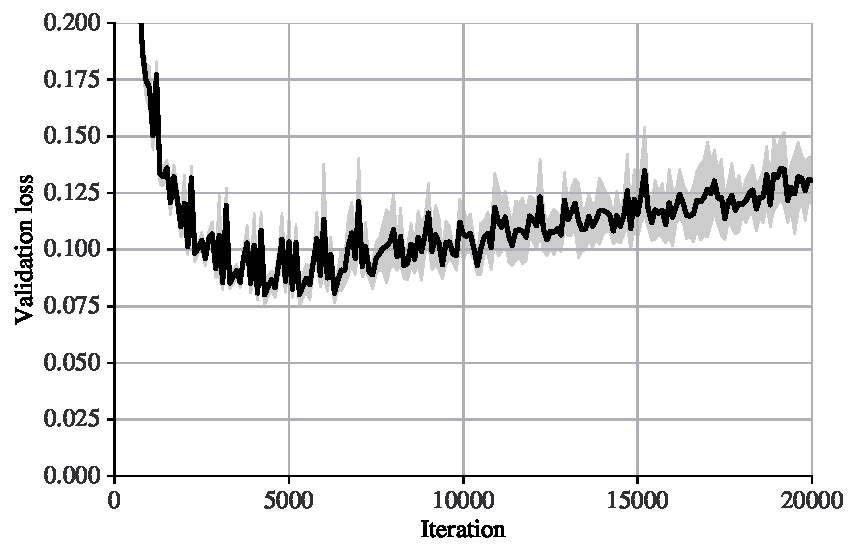
\includegraphics[width=0.75\textwidth]{plots/initial_trainings.pdf}
  \caption{The validation loss during the initial training run, evaluated every $100$ iterations across all ten random seeds. The indicated intervals show the standard deviation. Overfitting is clearly apparent: After about iteration $5000$, the validation starts increasing again.}
  \label{fig:initial-training}
\end{figure}

Because of this, we record at which iteration the minimal validation loss was achieved, and retrain the network from scratch -- starting from the saved, initial parameters -- for that many iterations. For all random seeds, the minimal validation loss is always achieved around iteration $5000$. While the training will never go exactly the same the second time around due to randomness, this seems to work well in practice both in our experiments and in \cite{supermask}, yielding a trained, non-overfit baseline network. The validation loss during the second training run is visualized in Figure \ref{fig:refined-training}.

Across random seeds, the validation accuracy is $0.101 \pm 0.016$ before training and $0.977 \pm 0.001$ after training, where the $\pm$ sign denotes the standard deviation.

\newpage

\begin{figure}[h!]
  \centering
  \textbf{Validation loss during refined training with early stopping}\par\medskip
  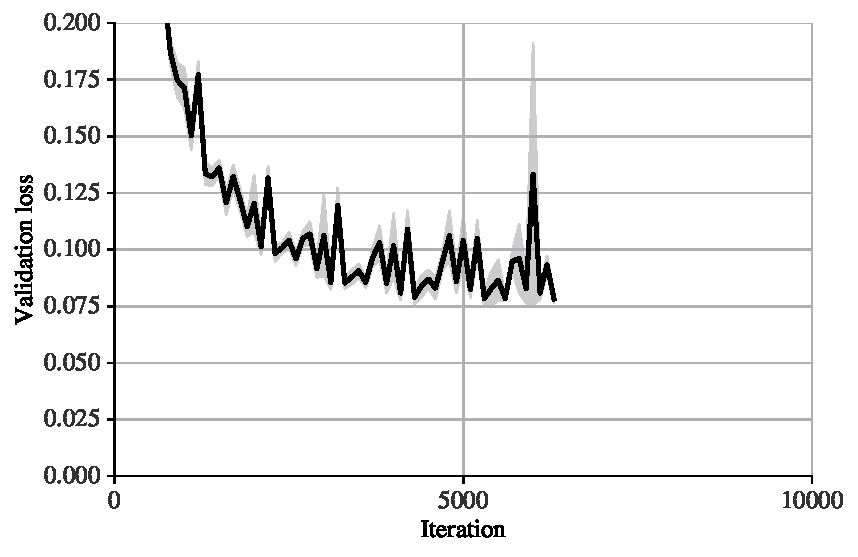
\includegraphics[width=0.75\textwidth]{plots/refined_trainings.pdf}
  \caption{The validation loss during the second training run with early stopping, evaluated every $100$ iterations across all ten random seeds. The indicated intervals show the standard deviation. For each seed, the training was stopped at the iteration that achieved the minimal validation loss during the initial training run. We can see that this approach results in a non-overfit, small validation loss when the training finishes.}
  \label{fig:refined-training}
\end{figure}

\begin{figure}[h!]
  \centering
  \textbf{Sizes of masked networks}\par\medskip
  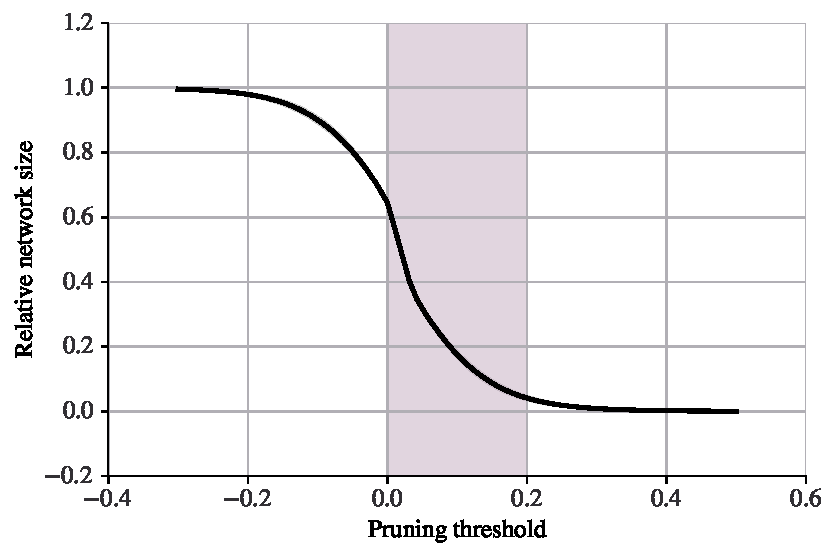
\includegraphics[width=0.75\textwidth]{plots/pruned_sizes.pdf}
  \caption{The relative network sizes after pruning with different tresholds. The variance across seeds is too small to be visible. The colored area indicates the tresholds that are considered as part of the evaluation of our methodology. }
  \label{fig:pruned-sizes}
\end{figure}

\begin{figure}[h]
  \centering
  \textbf{Validation accuracies of untrained masked networks}\par\medskip
  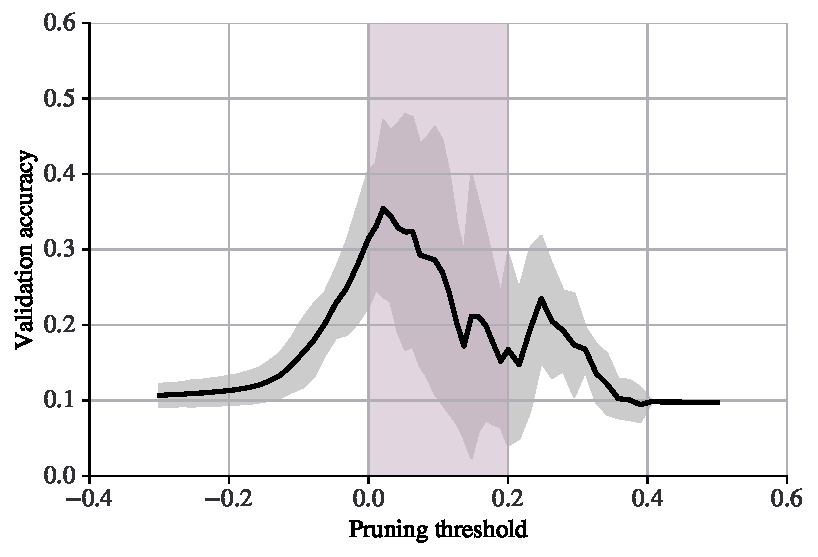
\includegraphics[width=0.75\textwidth]{plots/pruned_accuracies.pdf}
  \caption{The validation accuracies obtained when evaluating the untrained, masked networks for different tresholds, aggregated across all ten seeds. The indicated intervals show the standard deviation. The colored area indicates the tresholds that are considered as part of the evaluation of our methodology. Even though the masked networks were never trained explicitly, they reach an accuracy that is significantly better than chance.}
  \label{fig:pruned-accuracies}
\end{figure}

\subsection{Supermasks}

We are now at step three of our methodology: The computation of the masked networks. To do this, we consider tresholds $t$ from the set $\left\{0, 0.01, 0.02, \ldots, 0.2\right\}$. As described above, we then take the initial parameters of the network, and set some of them to zero, using the formula
$$
w_i^{\text{new}} := \begin{cases}
w_i^{\text{initial}} & \text{if } \operatorname{sign}\left(w_i^{\text{initial}} \right) \cdot w_i^{\text{trained}} \geq t, \\ 
0 & \text{otherwise.} \\
\end{cases}
$$

The exact size reduction achieved by choosing a particular threshold depends on the initialization, but the variance is low accross seeds: $t=0$ results in a relative size of $64.6\% \pm 0.4$, while $t=0.2$ results in $4.1\% \pm 0.6$. The size for different tresholds is visualized in Figure \ref{fig:pruned-sizes}.

With step four, we now choose the treshold which resulted in the highest validation accuracy, before any further training is done. Here, the variance is very high across seeds. The ideal treshold is found to be at $0.049 \pm 0.049$, resulting in a relative network size of $38.7\% \pm 17.9$. The resulting accuracy of these masked and otherwise untrained networks is $42.6\% \pm 15.2$, where the smallest value observed is $19.1\%$ and the largest is $70.0\%$. This astonishing fact marks our first reproduced result: As claimed in \cite{supermask}, the strategy of masking the initial, random values does indeed lead to a high accuracy, even though there is no explicit training of the masked networks involved. This is shown in Figure \ref{fig:pruned-accuracies}, where the accuracies obtained by pruning with different tresholds are visualized across seeds.

\begin{figure}[h]
  \centering
  \textbf{Validation loss of lottery tickets and hyperoptimizations}\par\medskip
  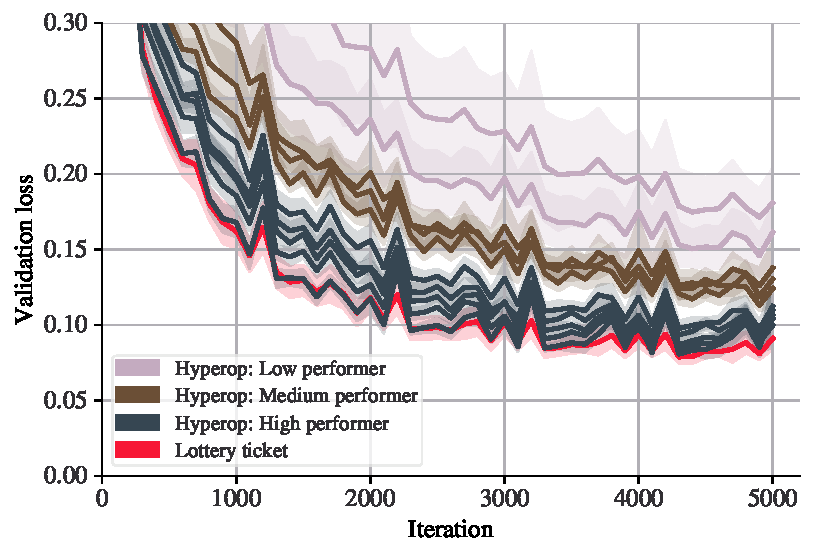
\includegraphics[width=0.75\textwidth]{plots/lt-loss.pdf}
  \caption{The validation loss during training of Lottery Tickets and hyperoptimized networks, evaluated every $100$ iterations across all ten random seeds. The indicated intervals show the standard deviation. The hyperoptimized networks were visually grouped into three categories based on their training performance. It is apparent that the performance of the Lottery Tickets is at least as good as all other hyperoptimizations.}
  \label{fig:lt-loss}
\end{figure}

\begin{figure}[h]
  \centering
  \textbf{Relative network sizes of lottery tickets and hyperoptimizations}\par\medskip
  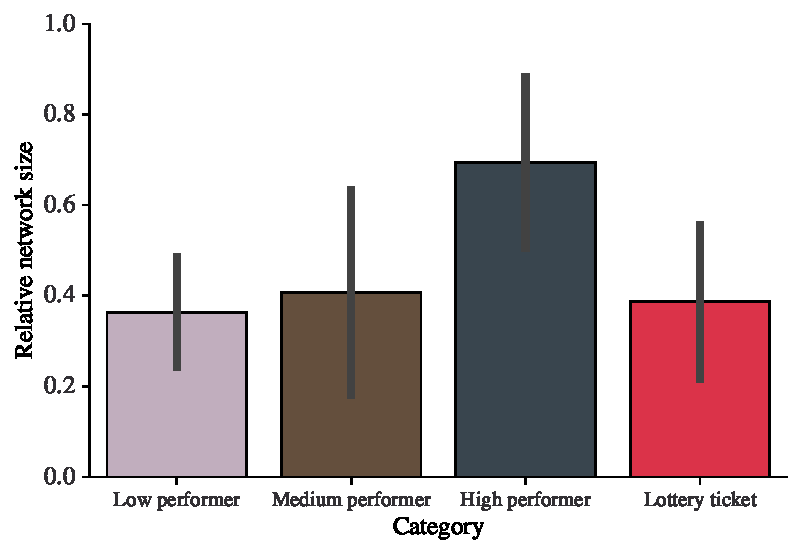
\includegraphics[width=0.75\textwidth]{plots/lt-size.pdf}
  \caption{The relative network sizes of the Lottery Tickets and the three groups of hyperoptimizations. The indicated intervals show the standard deviation. We can see that the Lottery Tickets are generally as small as the lowest performing hyperoptimizations.}
  \label{fig:lt-size}
\end{figure}

\subsection{Lottery tickets and hyperoptimization}
After having chosen a treshold using the Supermask evaluation, it is now time to train the corresponding masked network and thus create the "Lottery Ticket". This corresponds to steps 5 and 6 of our methodology. In order to have a good comparison for the newly created network's performance, we also use a simple hyperoptimization approach, which tries out smaller values for the baseline network's layer sizes. While the baseline uses sizes of $200$ and $30$ neurons for the first and second layers respectively, the hyperoptimization additionally considers all possible combinations of $(50, 100, 150)$ for the first layer and $(5, 15, 25)$ for the second layer. We are thus comparing the Lottery Ticket network to $1 + 3 \cdot 3 = 10$ other architectures.

To create the lottery ticket, we take the best-performing masked network from the previous step and train it for $5000$ iterations. We also train the ten different layer size configurations for $5000$ iterations, starting from random initializations. The validation loss for all these training runs is visualized in Figure \ref{fig:lt-loss} accross all seeds. We have grouped the different hyperoptimization into three groups by visually gauging their performance according to the graph. The graph shows that the lottery ticket trains at least as quickly and effectively as all the hyperoptimization approaches. After 5000 iterations, the lottery ticket achieves a validation loss of $0.091 \pm 0.007$ while the original baseline network architecture (without any layer size reduction) achieves $0.109 \pm 0.019$. The "High performer" group of hyperoptimizations as a whole achieves a final validation loss of $0.106 \pm 0.016$.

At the same time, the Lottery Ticket networks that were found by our method are generally smaller (pruned more aggressively) than the results from the hyperoptimization. This can be seen in Figure \ref{fig:lt-size}, which shows the relative network sizes of all the resulting networks. As described in the previous section, the optimal Supermasks, and therefore also the Lottery Tickets, have a relative network size of $38.7\% \pm 17.9$. Thus, our method produces networks that are comparable in size to the low-performing hyperoptimizations, while they tend to outperform even the high-performing hyperoptimizations. The detailed data for the validation losses and sizes of all the different architectures can be found in Table \ref{tab:lt-data}.

\begin{table}[p]
\resizebox{\textwidth}{!}{
\begin{tabular}{llllll}
\toprule
\thead[l]{Label} & \thead[l]{Category} &     \thead[l]{Relative size}  & \thead[l]{Final validation loss} & \thead[l]{Minimal validation loss} & \thead[l]{Iteration of minimal \\ validation loss}\\
\midrule
 Lottery ticket &  Lottery ticket &  $38.7\% \pm 17.9$ & $0.091 \pm 0.007$ &       $0.078 \pm 0.004$ &                   $4340.0 \pm 222.1$ \\
 Hyperop (200, 30) [baseline] &  High performer &  $100.0\%$  &     $0.109 \pm 0.019$ &       $0.078 \pm 0.001$ &                   $4360.0 \pm 171.3$\\
 Hyperop (100, 15) &  High performer &   $49.1\%$ &     $0.112 \pm 0.015$ &       $0.095 \pm 0.005$ &                   $4600.0 \pm 326.6$ \\
 Hyperop  (100, 25) &  High performer &   $49.8\%$  &     $0.104 \pm 0.008$ &       $0.090 \pm 0.003$ &                   $4540.0 \pm 340.6$\\
 Hyperop  (150, 15) &  High performer &   $73.6\%$ &     $0.106 \pm 0.021$ &       $0.085 \pm 0.003$ &                   $4660.0 \pm 275.7$ \\
 Hyperop  (150, 25) &  High performer &   $74.6\%$ &   $0.100 \pm 0.012$ &       $0.082 \pm 0.003$ &                   $4330.0 \pm 249.7$ \\
 Hyperop (50, 15) &  Medium performer &   $24.6\%$ &    $0.130 \pm 0.010$ &       $0.119 \pm 0.006$ &                   $4700.0 \pm 326.6$ \\
 Hyperop (50, 25) &  Medium performer &   $25.0\%$ &    $0.124 \pm 0.012$ &       $0.113 \pm 0.004$ &                    $4870.0 \pm 94.9$ \\
 Hyperop (150, 5) &  Medium performer &   $72.6\%$ &    $0.138 \pm 0.017$ &       $0.122 \pm 0.010$ &                   $4640.0 \pm 231.9$ \\
 Hyperop (100, 5) &  Low performer &   $48.4\%$ &    $0.161 \pm 0.019$ &       $0.146 \pm 0.014$ &                    $4870.0 \pm 94.9$ \\
 Hyperop (50, 5) &  Low performer &   $24.2\%$  &    $0.181 \pm 0.023$ &       $0.170 \pm 0.020$ &                   $4770.0 \pm 258.4$\\
\bottomrule
\end{tabular}
}
\caption{Comparison of performance and size between the Lottery Tickets and the hyperoptimized networks. ``Hyperop $(a, b)$'' indicates a network architecture with first layer size $a$ and second layer size $b$. All networks were trained for $5000$ iterations. The data indicates that the Lottery Tickets reach a better performance while having a smaller sizes than the hyperoptimized networks. }
\label{tab:lt-data}
\end{table}

\section{Conclusion}

Todo.
% todo: reproduction, but effect observed is not as strong

\newpage
%\fancyhead[LE]{\it \leftmark}
%\chapter{}
\fancyhead[LE,RO]{\it References}       % A bibliography never have a letter or numbering!
    \addcontentsline{toc}{section}{References}% Add to the TOC
    \printbibliography
%\cleardoublepage

\end{document}


% Fragen
% Wie viele Seiten?
% Wirklich nötig, erst approach, dann results? SChwierig zu erklären und komischer Fluss, den die Methodik baut ja auf den intermediate results auf
% Vielleicht mehrere results sections? 1. Reproduction of supermask performance, 1.1. Approach, 1.2. Results, then 2. Methodology for finding Lottery Tickets in practice

